% Copyright (C) 2010,2011 The ESPResSo project
% Copyright (C) 2002,2003,2004,2005,2006,2007,2008,2009,2010 
%   Max-Planck-Institute for Polymer Research, Theory Group
%  
% This file is part of ESPResSo.
%   
% ESPResSo is free software: you can redistribute it and/or modify it
% under the terms of the GNU General Public License as published by the
% Free Software Foundation, either version 3 of the License, or (at your
% option) any later version.
%  
% ESPResSo is distributed in the hope that it will be useful, but
% WITHOUT ANY WARRANTY; without even the implied warranty of
% MERCHANTABILITY or FITNESS FOR A PARTICULAR PURPOSE.  See the GNU
% General Public License for more details.
%  
% You should have received a copy of the GNU General Public License
% along with this program.  If not, see <http://www.gnu.org/licenses/>.
%
\chapter{Setting up particles}
\label{chap:part}

\section{\texttt{part}: Creating single particles}
\newescommand{part}

\subsection{Defining particle properties}

\begin{essyntax}
  part
  \var{pid}
  \opt{pos \var{x} \var{y} \var{z}}
  \opt{type \var{typeid}}
  \opt{v \var{vx} \var{vy} \var{vz}}
  \opt{f \var{fx} \var{fy} \var{fz}}
  \opt{bond \var{bondid} \var{pid2} \dots}
  \require{1}{\opt{q \var{charge}}}
  \require{2}{\opt{quat \var{q1} \var{q2} \var{q3} \var{q4}}}
  \require{2}{\opt{omega \var{x} \var{y} \var{z}}}
  \require{2}{\opt{torque \var{x} \var{y} \var{z}}}
  \require{2}{\opt{rinertia \var{x} \var{y} \var{z}}}
  \require{3}{\opt{\opt{un}fix \var{x} \var{y} \var{z}}}
  \require{3}{\opt{ext_force \var{x} \var{y} \var{z}}}
  \require{4}{\opt{exclude \var{pid2}\dots}}
  \require{4}{\opt{exclude delete \var{pid2}\dots}}
  \require{5}{\opt{mass \var{mass}}}
  \require{6}{\opt{dipm \var{moment}}}
  \require{6}{\opt{dip \var{dx} \var{dy} \var{dz}}}
  \require{7,8}{\opt{virtual \var{v}}}
  \require{8}{\opt{vs\_relative \var{pid} \par{distance}}}
  \require{8}{\opt{vs\_auto\_relate\_to \var{pid}}}
  \begin{features}
    \required[1]{ELECTROSTATICS} 
    \required[2]{ROTATION}
    \required[3]{EXTERNAL_FORCES}
    \required[4]{EXCLUSION}
    \required[5]{MASS}
    \required[6]{DIPOLES}
    \required[7]{VIRTUAL\_SITES\_COM}
    \required[8]{VIRTUAL\_SITES\_RELATIVE}
  \end{features}
\end{essyntax}

This command modifies particle data, namely position, type (monomer,
ion, \dots), charge, velocity, force and bonds. Multiple properties can
be changed at once. If you add a new particle the position has to be
set first because of the spatial decomposition.

\begin{arguments}
\item[\var{pid}]
\item[\opt{pos \var{x} \var{y} \var{z}}] Sets the position of this
  particle to $(x,y,z)$.
\item[\opt{type \var{typeid}}] Restrictions:
  $\var{typeid} \geq 0$.\\ The
  \var{typeid} is used in the \keyword{inter} command
  (see section \vref{tcl:inter}) to define the parameters of the non
  bonded interactions between different kinds of particles.
\item[\opt{v \var{vx} \var{vy} \var{vz}}] Sets the velocity of
this particle to $(vx,vy,vz)$. The velocity remains variable and will be changed
during integration.
\item[\opt{f \var{fx} \var{fy} \var{fz}}] Set the force acting on this particle
to $(fx,fy,fz)$. The force remains variable and will be changed during integration.
\item[\opt{bond \var{bondid} \var{pid2}\dots}]
  Restrictions: \var{bondid} $\geq 0$; \var{pid2} must
  be an existing particle.  The \var{bondid} is used for
  the inter command to define bonded interactions.
\item[bond delete] Will delete all bonds attached to this particle.
\item[\opt{q \var{charge}}] Sets the charge of this particle to $q$.
\item[\opt{quat \var{q1} \var{q2} \var{q3} \var{q4}}] Sets the
  quaternion representation of the rotational position of this
  particle.
\item[\opt{omega \var{x} \var{y} \var{z}}] Sets the rotational velocity of this particle in global frame.
\item[\opt{torque \var{x} \var{y} \var{z}}] Sets the rotational force of this particle, in global frame.
  When printing the values using {\em part id_particle print}, there is an alternative named
  \opt{tbf} which gives you the values of the torque in the body frame.  Be aware: the values obtained when printing using \opt{torque}
  are computed in the frame laboratory and are the ones one should usually look at. Nonetheless,  in case you 
  introduce torques using \opt{torque} option, espresso will assume they are given in the body-frame. Thus \opt{tbf} is useful
  to know which should be the numerical values you should reintroduce in order to have exactly the same conformation.
\item[\opt{rinertia \var{x} \var{y} \var{z}}] Sets the diagonal
    elements of this particles rotational inertia.
\item[\opt{fix \var{x} \var{y} \var{z}}] Fixes the particle in space.
  By supplying a set of 3 integers as arguments it is possible to fix
  motion in \var{x}, \var{y}, or \var{z} coordinates independently. For
  example \var{fix 0 0 1} will fix motion only in z. Note that
  \var{fix} without arguments is equivalent to \var{fix 1 1 1}.
\item[\opt{ext_force \var{x} \var{y} \var{z}}]
  An additional external force is applied to the particle.
\item[\opt{unfix}] Release any external influence from the particle.
\item[\opt{exclude \var{pid2}\dots+}] Restrictions:
  \var{pid2} must be an existing particle.  Between the
  current particle an the exclusion partner(s), no nonbonded
  interactions are calculated. Note that unlike bonds, exclusions are
  stored with both partners.  Therefore this command adds the defined
  exclusions to both partners.
\item[\opt{exclude delete \var{pid2}\dots}] Searches for the
  given exclusion and deletes it. Again deletes the exclusion with
  both partners.
  \item[\opt{mass \var{mass}}] Sets the mass of this particle to $mass$. If not
  set, all particles have a mass of 1 in reduced units.
  \item[\opt{dipm \var{moment}}] Sets the dipol moment of this particle to $moment$.
  \item[\opt{dip \var{dx} \var{dy} \var{dz}}] Sets the orientation of the
  dipol axis to $(dx,dy,dz)$.
\item[\opt{virtual \var{v}}] Declares the particles as virtual (1) or
  non-virtual (0, default). Please read chapter \ref{sec:virtual}
  before using virtual sites.
\item[\opt{vs\_auto\_relate\_to \var{pid}}] Automatically relates a
  virtual site to a non-virtual particle for the ``relative''
  implementation of virtual sites. \var{pid} is the id of the particle
  to which the virtual site should be related.
\item[\opt{vs\_relative \var{pid} \var{distance}}] Allows for manual
  access to the attributes of virtual sites in the ``relative''
  implementation. \var{pid} denotes the id of the particle to which
  this virtual site is related and \var{distance} the distance between
  non-virtual and virtual particle.
   \end{arguments}

\subsection{Getting particle properties}

\begin{essyntax}
  \variant{1}
  part \var{pid} print
  \optlong{\alt{id \asep pos \asep type \asep folded_position \asep type \asep
      q \asep v \asep f \asep fix \asep ext_force \asep bond \asep
      \mbox{connections \opt{\var{range}}}}}\dots
  \variant{2} part
\end{essyntax}

Variant \variant{1} will return a list of the specified properties of
particle \var{pid}, or all properties, if no keyword is
specified.  Variant \variant{2} will return a list of all properties
of all particles.

\minisec{Example}
\begin{code}
part 40 print id pos q bonds
\end{code}
will return a list like
\begin{tclcode}
40 8.849 1.8172 1.4677 1.0 {}
\end{tclcode}
This routine is primarily intended for effective use in Tcl scripts.

When the keyword \keyword{connection} is specified, it returns the
connectivity of the particle up to \var{range} (defaults to 1). For
particle 5 in a linear chain the result up to \var{range} = 3 would
look like:
\begin{tclcode}
{ { 4 } { 6 } } { { 4 3 } { 6 7 } } { {4 3 2 } { 6 7 8 } } 
\end{tclcode}
The function is useful when you want to create bonded interactions to
all other particles a certain particle is connected to. Note that this
output can not be used as input to the part command. Check results if
you use them in ring structures.

If none of the options is specified, it returns all properties of the
particle, if it exists, in the form
\begin{tclcode}
  0 pos 2.1 6.4 3.1 type 0 q -1.0 v 0.0 0.0 0.0 f 0.0 0.0 0.0
  bonds { {0 480} {0 368} ... } 
\end{tclcode}
which may be used as an input to this function later on. The first
integer is the particle number.

Variant \variant{2} returns the properties of all stored particles in
a tcl-list with the same format as specified above:
\begin{tclcode}
{0 pos 2.1 6.4 3.1 type 0 q -1.0 v 0.0 0.0 0.0 f 0.0 0.0 0.0
 bonds{{0 480}{0 368}...}} 
{1 pos 1.0 2.0 3.0 type 0 q 1.0 v 0.0 0.0 0.0 f 0.0 0.0 0.0
 bonds{{0 340}{0 83}...}} 
{2...{{...}...}}
{3...{{...}...}}
...
\end{tclcode}

\subsection{Deleting  particles}
\label{tcl:part:delete}

\begin{essyntax}
  \variant{1} part \var{pid} delete
  \variant{2} part deleteall
\end{essyntax}

In variant \variant{1}, the particle \var{pid} is deleted
and all bonds referencing it.  Variant \variant{2} will delete all
particles currently present in the simulation. Variant \variant{3}
will delete all currently defined exclusions.

\subsection{Exclusions}

\begin{essyntax}
  \variant{1} part auto\_exclusions \opt{\var{range}}
  \variant{2} part delete\_exclusions
  \begin{features}
    \required{EXCLUSIONS} 
  \end{features}
\end{essyntax}


Variant \variant{1} will create exclusions for all particles pairs
connected by not more than \var{range} bonds (\var{range} defaults to
2). This is typically used in atomistic simulations, where nearest and
next nearest neighbour interactions along the chain have to be omitted
since they are included in the bonding potentials. For example, if the
system contains particles $0$ \dots $100$, where particle $n$ is
bonded to particle $n-1$ for $1 \leq n \leq 100$, then it will result
in the exclusions:
\begin{itemize}
  \item particle 1 does not interact with particles 2 and 3
  \item particle 2 does not interact with particles 1, 3 and 4
  \item particle 3 does not interact with particles 1, 2, 4 and 5
  \item ...
\end{itemize}

Variant \variant{2} deletes all exclusions currently present in the
system.

\section{Creating groups of particle}

\subsection{\texttt{polymer}: Setting up polymer chains}

\newescommand{polymer}
\begin{essyntax}
  polymer 
  \var{num\_polymers} \var{monomers\_per\_chain}
  \var{bond\_length}\\
  \opt{start \var{pid}} 
  \opt{pos \var{x} \var{y} \var{z}}
  \opt{mode \alt{RW \asep SAW \asep PSAW} 
    \opt{\var{shield} \opt{\var{try_\mathrm{max}}}}} 
  \require{1}{\opt{charge \var{q}}} 
  \require{1}{\opt{distance \var{d_\mathrm{charged}}}}
  \opt{types \var{typeid_\mathrm{neutral}}
    \opt{\var{typeid_\mathrm{charged}}}} 
  \opt{bond \var{bondid}} 
  \opt{angle \var{\phi} \opt{\var{\theta} \opt{\var{x} \var{y}
        \var{z}}}}
  \require{2}{\opt{constraints}}
  \begin{features}
    \required[1]{ELECTROSTATICS}
    \required[2]{CONSTRAINTS}
  \end{features}
\end{essyntax}

This command will create \var{num\_polymers} polymer or
polyelectrolyte chains with \var{monomers\_per\_chain} monomers per
chain. The length of the bond between two adjacent monomers will be
set up to be \var{bond\_length}.

\begin{arguments}
\item[\var{num\_polymers}] Sets the number of polymer chains.
\item[\var{monomers\_per\_chain}] Sets the number of monomers per
  chain.
\item[\var{bond\_length}] Sets the initial distance between two adjacent
  monomers. The distance during the course of the simulation depends on the
  applied potentials. For fixed bond length please refer to the SHAKE algorithm.
  \todo{Link to rattle/shake.}
\item[\opt{start \var{pid}}] Sets the particle number of the
  start monomer to be used with the \keyword{part} command. This
  defaults to 0.

\item[\opt{pos \var{x} \var{y} \var{z}}] Sets the position of the
  first monomer in the chain to \var{x}, \var{y}, \var{z} (defaults to
  a randomly chosen value)
  
\item[\opt{mode \alt{RW  \asep  PSAW  \asep  SAW} \opt{\var{shield}
      \opt{\var{try_\mathrm{max}}}}}]
  Selects the setup mode:
  \begin{description}
  \item[\keyword{RW} (Random walk)] The monomers are
    randomly placed by a random walk with a steps size of
    \var{bond_length}.
  \item[\keyword{PSAW} (Pruned self-avoiding walk)] The position of a
    monomer is randomly chosen in a distance of \var{bond\_length} to
    the previous monomer. If the position is closer to another
    particle than \var{shield}, the attempt is repeated up to
    \var{try_\mathrm{max}} times. Note, that this is not a real
    self-avoiding random walk, as the particle distribution is not the
    same. If you want a real self-avoiding walk, use the \keyword{SAW}
    mode.  However, \keyword{PSAW} is several orders of magnitude
    faster than \keyword{SAW}, especially for long chains.
  \item[\keyword{SAW} (Self-avoiding random walk)] The positions of
    the monomers are chosen as in the plain random walk. However, if
    this results in a chain that has a monomer that is closer to
    another particle than \var{shield}, a new attempt of setting up
    the whole chain is done, up to \var{try_\mathrm{max}} times.
  \end{description}
  The default for the mode is \keyword{RW}, the default for the
  \var{shield} is $1.0$, and the default for \var{try_\mathrm{max}} is
  $30000$, which is usually enough for \keyword{PSAW}. Depending on
  the length of the chain, for the \keyword{SAW} mode,
  \var{try_\mathrm{max}} has to be increased by several orders of
  magnitude.
\item[\opt{charge \var{valency}}] Sets the valency of the charged
  monomers.  If the valency of the charged polymers \var{valency} is
  smaller than $10^{-10}$, the charge is assumed to be zero, and the
  types are set to $\var{typeid_\mathrm{charged}} =
  \var{typeid_\mathrm{neutral}}$. If charge is not set, it defaults to
  0.0.
\item[\opt{distance \var{d_\mathrm{charged}}}] Sets the stride
  between the indices of two charged monomers. This defaults defaults
  to 1, meaning that all monomers in the chain are charged.
\item[\opt{types \var{typeid_\mathrm{neutral}}
    \var{typeid_\mathrm{charged}}}] Sets the type ids of the neutral
    and charged monomer types to be used with the \keyword{part}
    command. If only \var{typeid_\mathrm{neutral}} is defined,
    \var{typeid_\mathrm{charged}} defaults to $1$. If the option is
    omitted, both monomer types default to $0$.
  \item[\opt{bond \var{bondid}}] Sets the type number of the bonded
    interaction to be set up between the monomers. This defaults to
    $0$.  Any bonded interaction, no matter how many bonding-partners
    needed, is stored with the second particle in this bond. See
    chapter \ref{sec:inter-bonded}.
  \item[\opt{angle \var{\phi} [\var{\theta} [\var{x} \var{y}
      \var{z}]]}] Allows for setting up helices or planar polymers:
    \var{\phi} and \var{theta} are the angles between adjacent bonds.
    \var{x}, \var{y} and \var{z} set the position of the second
    monomer of the first chain.
  \item[\opt{constraints}] If this option is specified, the particle setup-up
  tries to obey previously defined constraints (see section \vref{sec:constraint}).
\end{arguments}

\subsection{\texttt{counterions}: Setting up counterions}
\newescommand{counterions}
\begin{essyntax}
  counterions
  \var{N} 
  \opt{start \var{pid}} 
  \opt{mode \alt{SAW \asep RW} \opt{\var{shield} \opt{\var{try_\mathrm{max}} }}} 
  \require{1}{\opt{charge \var{val}}}
  \opt{type \var{typeid}}
  \begin{features}
    \required[1]{ELECTROSTATICS}
  \end{features}
\end{essyntax}
This command will create \var{N} counterions in the simulation box.
\begin{arguments}
\item[\opt{start \var{pid}}] Sets the particle id of the first
  counterion.  It defaults to the current number of particles, \ie
  counterions are placed after all previously defined particles.
\item[\opt{mode \alt{SAW \asep RW} \opt{\var{shield}
      \opt{\var{try_\mathrm{max}} }}}] Specifies the setup method to
  place the counterions. It defaults to \keyword{SAW}. See the
  \keyword{polymer} command for a detailed description.
\item[\opt{charge \var{val}}] Specifies the charge of the counterions.
  If not set, it defaults to $-1.0$.
\item[\opt{type \var{typeid}}] Specifies the particle type of the
  counterions. It defaults to $2$.
\end{arguments}

\smallskip
\subsection{\texttt{salt}: Setting up salt ions}
\newescommand{salt}
\begin{essyntax}
  salt 
  \var{N_+} \var{N_-} 
  \opt{start \var{pid}} 
  \opt{mode \alt{SAW \asep RW} \opt{\var{shield} \opt{\var{try_\mathrm{max}}}}}
  \require{1}{\opt{charges \var{val_+} \opt{\var{val_-}}}} 
  \opt{types \var{typeid_+} \opt{\var{typeid_-}}}
  \opt{rad \var{r}}
  \begin{features}
    \required[1]{ELECTROSTATICS}
  \end{features}
\end{essyntax}

Create \var{N_+} positively and \var{N_-} negatively charged salt ions
of charge \var{val_+} and \var{val_-} within the simulation box.
\begin{arguments}
\item[\opt{start \var{pid}}] Sets the particle id of the first
  (positively charged) salt ion. It defaults to the current number of
  particles.
\item[\opt{mode \alt{SAW \asep RW} \opt{\var{shield}
      \opt{\var{try_\mathrm{max}} }}}] Specifies the setup method to
  place the counterions. It defaults to \keyword{SAW}. See the
  \keyword{polymer} command for a detailed description.
\item[\opt{charge \var{val_+} \opt{\var{val_-}}}] Sets the charge of
  the positive salt ions to \var{val_+} and the one of the negatively
  charged salt ions to \var{val_-}. If not set, the values default to
  $1.0$ and $-1.0$, respectively.
\item[\opt{type \var{typeid_+} \opt{\var{typeid_-}}}] Specifies the
  particle type of the salt ions. It defaults to $3$ respectively $4$.
\item[\opt{rad \var{r}}] The salt ions are only placed in a
  sphere with radius \var{r} around the origin.
\end{arguments}


\subsection{\texttt{diamond}: Setting up diamond polymer networks}
\newescommand{diamond}
\begin{essyntax}
  diamond 
  \var{a} \var{bond\_length} \var{monomers\_per\_chain} 
  \opt{counterions \var{N_\mathrm{CI}}}\\ 
  \require{1}{\opt{charges \var{val_\mathrm{node}}
      \var{val_\mathrm{monomer}} \var{val_\mathrm{CI}}}}
  \require{1}{\opt{distance \var{d_\mathrm{charged}}}}
  \opt{nonet}
  \begin{features}
    \required[1]{ELECTROSTATICS}
  \end{features}
\end{essyntax}

Creates a diamond-shaped polymer network with 8 tetra-functional nodes
connected by $2*8$ polymer chains of length \var{monomers\_per\_chain} in 
a unit cell of length \var{a}. Chain monomers are placed at a mutual distance \var{bond\_length}
along the vector connecting network nodes.
The polymer is created starting from particle ID 0. Nodes are assigned type 0,
monomers (both charged and uncharged) are type 1 and counterions type 2.
For inter-particle bonds interaction $0$ is taken which must be a two-particle bond.

\begin{figure}[h]
  \label{fig:diamond}
  \begin{center}
  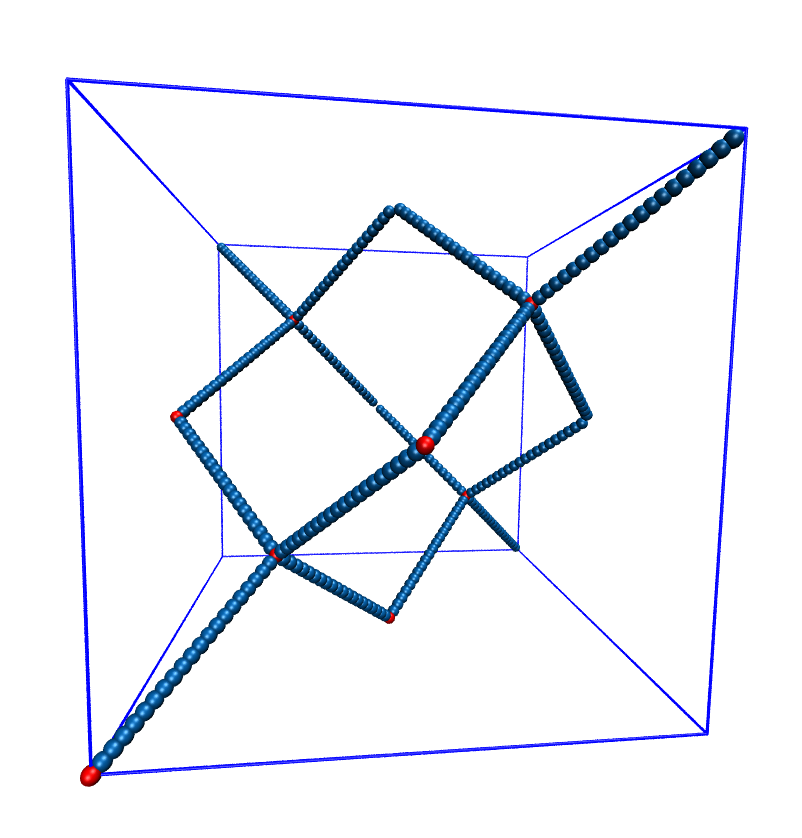
\includegraphics[height=6cm]{figures/diamond}
  \caption{Diamond-like polymer network with \var{monomers\_per\_chain}=15.}
  \end{center}
\end{figure}

\begin{arguments}
\item[\var{a}] Determines the size of the of the unit cell.
\item[\var{bond\_length}] Specifies the bond length of the polymer
  chains connecting the 8 tetra-functional nodes.
\item[\var{monomers\_per\_chain}] Sets the number of chain monomers
  between the functional nodes.
\item[\opt{counterions \var{N_\mathrm{CI}}}] Adds \var{N_\mathrm{CI}}
  counterions to the system.
\item[\opt{charges \var{val_\mathrm{node}} \var{val_\mathrm{monomer}}
    \var{val_\mathrm{CI}}}] Sets the charge of the nodes to
  \var{val_\mathrm{node}}, the charge of the connecting monomers to
  \var{val_\mathrm{monomer}}, and the charge of the counterions to
  \var{val_\mathrm{CI}}.
\item[\opt{distance \var{d_\mathrm{charged}}}] Specifies the distance
  between charged monomers along the interconnecting chains. If
  $\var{d_\mathrm{charged}} > 1$ the remaining chain monomers are
  uncharged.
  \item[\opt{nonet}] Do not create bonds between the chains.
\end{arguments}


\subsection{\texttt{icosaeder}: Setting up an icosaeder}
\newescommand{icosaeder}
\begin{essyntax}
  icosaeder 
  \var{a} \var{monomers\_per\_chain} 
  \opt{counterions \var{N_\mathrm{CI}}} 
  \require{1}{\opt{charges \var{val_\mathrm{monomers}} \var{val_\mathrm{CI}}}}
  \require{1}{\opt{distance \var{d_\mathrm{charged}}}}
  \begin{features}
    \required[1]{ELECTROSTATICS}
  \end{features}
\end{essyntax}

Creates a modified icosaeder to model a fullerene (or soccer ball).
The edges are modeled by polymer chains connected at the corners of
the icosaeder. For inter-particle bonds interaction $0$ is taken which
must be a two-particle bond. Two particle types are used for the
pentagons and the interconnecting links. For an example, see figure \ref{fig:fullerene}.

\begin{figure}[h]
  \label{fig:diamond}
  \begin{center}
  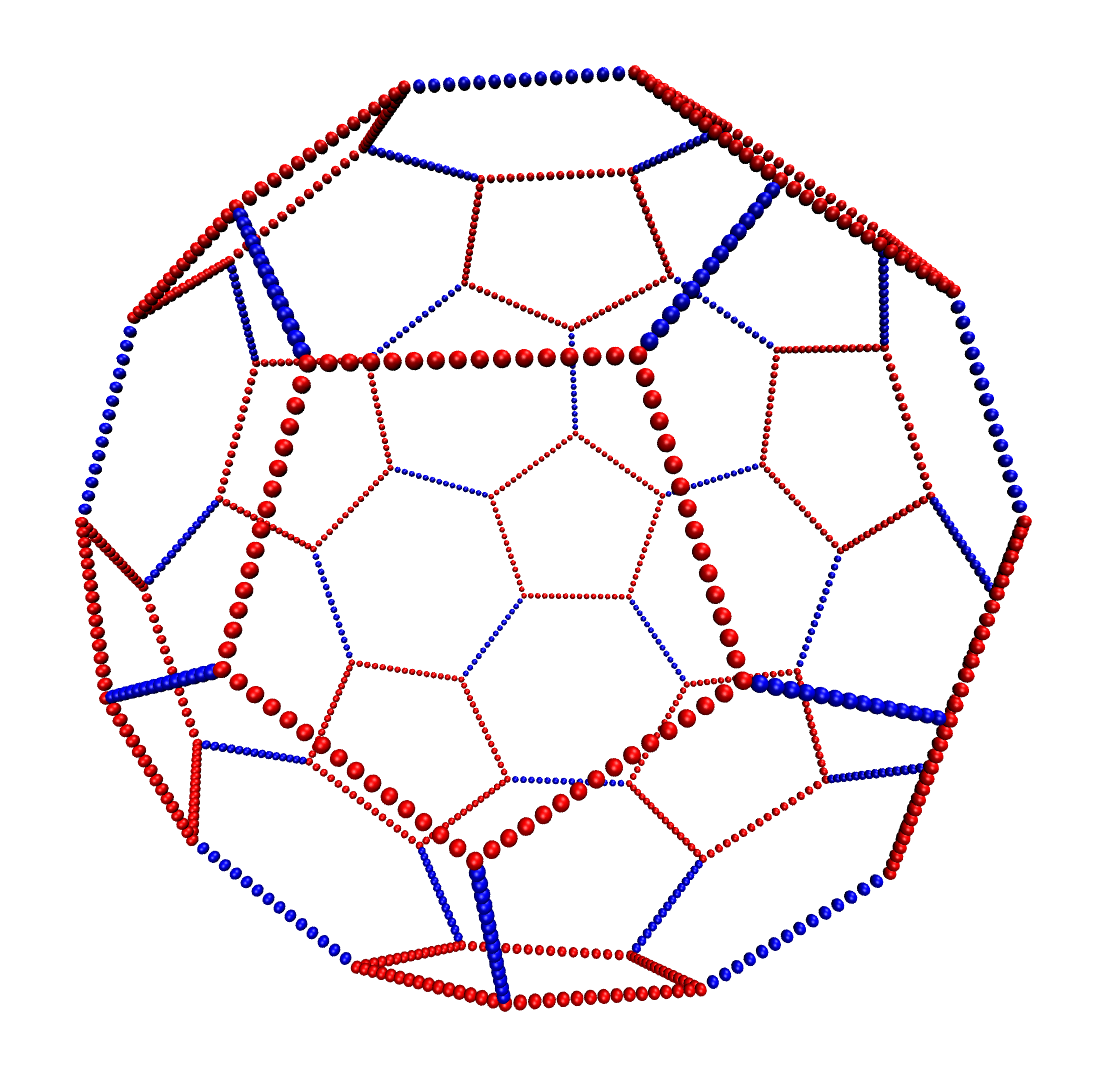
\includegraphics[height=6cm]{figures/fullerene}
  \caption{Icosaeder with \var{monomers\_per\_chain}=15.}
  \label{fig:fullerene}
  \end{center}
\end{figure}

\begin{arguments}
\item[\var{a}] Length of the links. Defines the size of the icosaeder.
\item[\var{monomers\_per\_chain}] Specifies the number of chain monomers along one edge.
\item[\opt{counterions \var{N_\mathrm{CI}}}] Specifies the number of
  counterions to be placed into the system.
\item[\opt{charges \var{val_\mathrm{monomers}} \var{val_\mathrm{CI}}}]
  Set the charges of the monomers to \var{val_\mathrm{monomers}} and
  the charges of the counterions to \var{val_\mathrm{CI}}.
\item[\opt{distance \var{d_\mathrm{charged}}}] Specifies the distance
  between two charged monomer along the edge. If
  $\var{d_\mathrm{charged}} > 1$ the remaining monomers are uncharged.
\end{arguments}

\subsection{\texttt{crosslink}: Cross-linking polymers}
\newescommand{crosslink}
\begin{essyntax}
  crosslink 
  \var{num\_polymer} \var{monomers\_per\_chain} 
  \opt{start \var{pid}} 
  \opt{catch \var{r_\mathrm{catch}}}
  \opt{distLink \var{link\_dist}} 
  \opt{distChain \var{chain\_dist}} 
  \opt{FENE \var{bondid}} 
  \opt{trials \var{try_\mathrm{max}}} 
\end{essyntax}

Attempts to end-crosslink the current configuration of
\var{num\_polymer} equally long polymers with
\var{monomers\_per\_chain} monomers each, returning how many ends are
successfully connected.

\begin{arguments}
\item[\opt{start \var{pid}}] \var{pid} specifies the first monomer of
  the chains to be linked. It has to be specified if the polymers do
  not start at id 0.
\item[\opt{catch \var{r_catch}}] Set the radius around each monomer
  which is searched for possible new monomers to connect to.
  \var{r_\mathrm{catch}} defaults to $1.9$.
\item[\opt{distLink \var{link\_dist}}] The minimal distance of two
  interconnecting links. It defaults to $2$.
\item[\opt{distChain \var{chain\_dist}}] The minimal distance for an
  interconnection along the same chain. It defaults to $0$. If set to
  \var{monomers\_per\_chain}, no interchain connections are created.
\item[\opt{FENE \var{bondid}}] Sets the bond type for the connections
  to \var{bondid}.
\item[\opt{trials \var{try_\mathrm{max}}}] If not specified,
  \var{try_\mathrm{max}} defaults to $30000$.
\end{arguments}

\subsection{\texttt{copy\_particles}: copying a set of particles}
\newescommand[copy-particles]{copy\_particles}
\begin{essyntax}
  copy_particles
  \opt{set \var{id1} \var{id2} \dots \asep range \var{from} {to} \dots} 
  \opt{shift \var{s\_x} \var{s\_y} \var{s\_z}}
\end{essyntax}

Copy a group of particles including their bonds. Positions can be
\opt{shift}ed by an offset $(\var{s\_x}, \var{s\_y}, \var{s\_z})$,
otherwise the copied set is at exactly the same position as the
original set. The particles can be given as a combination of
\opt{list}s or \opt{range}s. The new particles obtain in any case
consecutive identities after the largest current identity. Bonds
within the defined particle set are copied with translated identities,
but not bonds with particles outside the list. That is, if the
particle set corresponds to a molecule, intramolecular bonds are
preserved, but not intermolecular ones.

Examples of use:\\
\begin{tclcode}
  copy_particles set {1 2 3 4} shift 0.0 0.0 0.0
  copy_particles set {1 2} set {3 4}
  copy_particles range 1 4
\end{tclcode}
All these examples do the same - making exact copies of particles 1 through 4.

\section{\texttt{constraint}: Setting up constraints}\label{sec:constraint}
\newescommand{constraint}

\begin{essyntax}
  \variant{1} 
  constraint wall normal \var{n_x} \var{n_y} \var{n_z} 
  dist \var{d} type \var{id} \opt{penetrable \var{flag}} \opt{reflecting \var{flag}}
  
  \variant{2}
  constraint sphere center \var{c_x} \var{c_y} \var{c_z} 
  radius \var{rad} direction \var{direction} type \var{id} \opt{penetrable \var{flag}} \opt{reflecting \var{flag}}
  
  \variant{3}
  constraint cylinder center \var{c_x} \var{c_y} \var{c_z} 
  axis \var{n_x} \var{n_y} \var{n_z} 
  radius \var{rad} length \var{length} 
  direction \var{direction} 
  type \var{id}  \opt{penetrable \var{flag}} \opt{reflecting \var{flag}}
  
  \variant{4}
  constraint maze nsphere \var{n} 
  dim \var{d} sphrad \var{r_s} cylrad \var{r_c}
  type \var{id} \opt{penetrable \var{flag}}
  
  \variant{5}  
  constraint pore center \var{c_x} \var{c_y} \var{c_z} 
  axis \var{n_x} \var{n_y} \var{n_z} 
  radius \var{rad} length \var{length} 
  type \var{id} 
  
  \require{1}{%
    \variant{6}
    constraint rod center \var{c_x} \var{c_y} 
    lambda \var{lambda}
  } 
  
  \require{1}{%
    \variant{7}
    constraint plate height \var{h}
    sigma \var{sigma} 
  }
  
  \require{2,3}{%
    \variant{8}
    constraint ext_magn_field \var{f_x} \var{f_y} \var{f_z} 
  }
  
  \variant{9} 
  constraint plane cell \var{x} \var{y} \var{z} 
  type \var{id}

  \variant{10}
  constraint mindist_position \var{x} \var{y} \var{z} 

  \begin{features}
    \required{CONSTRAINTS}
    \required[1]{ELECTROSTATICS}
    \required[2]{ROTATION}
    \required[3]{DIPOLES}
  \end{features}
\end{essyntax}

The \codebox{constraint} command offers a variety of surfaces that can be
defined to interact with desired particles. Variants \variant{1} to \variant{5}
create interactions via a non-bonded interaction potential, where the distance
between the two particles is replaced by the
distance of the center of the particle to the surface. The constraints are
identified like a particle via its type for the non-bonded interaction. 
After a type is defined for each constraint one has
to define
the interaction of all different particle types with the constraint using
the \codebox{inter} command. In variants \variant{1} to \variant{4}, constraints
 are able to be penetrated if \var{flag} is set to 1. Otherwise, when the
 penetrable option is ignored or \var{flag} is set to 0, the constraint
 cannot be violated, i.e. no particle can go through the constraint surface.
 In variants \variant{1} to \variant{3} it is also possible to specify a flag 
 indicating if the constraints should be reflecting. The flags can equal 1 or 2.
 The flag 1 corresponds to a reflection process where the normal component of the 
 velocity is reflected and the tangential component remains unchanged. If the
 flag is 2, also the tangential component is turned around, so that a bounce back
 motion is performed. The second variant is useful for boundaries of DPD.
 The reflection property is only activated if an interaction is defined between
 a particular particle and the constraint! This will usually be a lennard-jones
 interaction with $\epsilon=0$, but finite interaction range.

Variants \variant{6} and \variant{7} create interactions based on electrostatic
interactions. The corresponding force acts in direction of the normal vector of the
surface and applies to all charged particles.

Variant \variant{8} does not define a surface but is based on magnetic
dipolar interaction with an external magnetic field. It applies to all particles
with a dipol moment.

Variant \variant{9} is essential for the use of tunable-slip boundary
interactions for microchannel flows like the Plane Poiseuille or Plane Couette
Flow.

Variant \variant{10} calculates the smallest distance to all non-penetrable
constraints, that can be repulsive (wall, cylinder, sphere, maze, pore).
Negative distances mean that the position is ``within'' the area that
particles should not access. Helpful to find initial configurations.) 

\textbf{Note that constraints are not saved to checkpoints and that they have to
be reset upon restarting a simulation.}

The resulting surface in variant \variant{1} is a plane defined by the
normal vector \var{n_x} \var{n_y} \var{n_z} and the distance
\var{d} from the origin. The force acts in direction of the normal. 
Note that the \var{d} describes the distance from the origin in units
of the normal vector so that the product of $d$ and $n$ is a point on the
surface. Therefore negative distances are quite common!

The resulting surface in variant
\variant{2} is a sphere with center \var{c_x} \var{c_y} \var{c_z} and radius
\var{rad}. The \var{direction} determines the force direction, -1 or
\opt{inside} for inward and +1 or \opt{outside} for outward. 

The resulting surface
in variant \variant{3} is a cylinder with center \var{c_x} \var{c_y}
\var{c_z} and radius \var{rad}. The \var{length} parameter is \textbf{half} 
of the cylinder length. The \var{axis} is a
vector along the cylinder axis, which is normalized in the program.
The \var{direction} is defined the same way as for the spherical
constraint. 

The resulting surface in variant \variant{4} is \var{n}
spheres of radius \var{r_s} along each dimension, connected by
cylinders of radius \var{r_c}. The spheres have simple cubic
symmetry. The spheres are distributed evenly by dividing the
\var{box_l} by \var{n}.  Dimension of the maze can be controlled by
\var{d}: 0 for one dimensional, 1 for two dimensional and 2 for three
dimensional maze.

Variant \variant{5} sets up a cylindrical pore similar to variant
\variant{3} with a center \var{c_x} \var{c_y} \var{c_z} and radius
\var{rad}. The \var{length} parameter is \textbf{half} of the cylinder
length. The \var{axis} is a vector along the cylinder axis, which is
normalized in the program. The argument \codebox{radius \var{rad}} 
can be replaced by the argument \codebox{ radii \var{rad1} \var{rad2}}
to obtain a pore with a conical shape and corresponding opening radii.
The first radius is in the direction opposite to the axis vector.

Variant \variant{6} specifies an electrostatic interaction between the
charged particles in the system to an infinitely long rod with a line
charge of \var{lambda} which is alinge along the z-axis and centered
at \var{c_x} and \var{c_y}.

Variant \variant{7} specifies the electrostatic interactinos between
the charged particles in the system and an inifinitely large plate in
the x-y-plane at height \var{h}. The plate carries a charge density of
\var{sigma}.
  
Variant \variant{8} specifies the dipolar coupling of particles with a
dipolar moment to an external field \var{f_x} \var{f_y} \var{f_z}.

Variant \variant{9} creates an infinite plane at a fixed position. For
non-initializing a direction of the constraint values of the positions
have to be negative. For the tunable-slip boundary interactions you
have to set \emph{two} constraints.

\minisec{Example}
To create an infinite plane in $z$-direction at $z=20.0$ of type id 1,
use:
\begin{code}
  constraint plane cell -10 -10 20 type 1
\end{code}

\subsection{Deleting a constraint}
\begin{essyntax}
  constraint delete \opt{\var{num}} 
\end{essyntax}

This command will delete constraints. If \var{num} is specified only this
constraint will deleted, otherwise all constraints will be removed from the
system. 

\subsection{Getting the force on a constraint}
\begin{essyntax}
constraint force \var{n} 
\end{essyntax}
Returns the force acting on the \var{n}th constraint.


\subsection{Getting the currently defined constraints}
\begin{essyntax}
constraint  \opt{\var{num}} 
\end{essyntax}
Prints out all constraint information. If \var{num} is specified only this
constraint is displayed, otherwise all constraints will be printed.

\section{Virtual sites}
\label{sec:virtual}
\index{virtual sites|mainindex}

Virtual sites are particles, the positions and velocities of which are
not obtained by integrating an equation of motion.  Rather, their
coordinates are obtained from the position (and orientation) of one or
more other particles. In this way, rigid arrangements of particles can
be constructed and a particle can be placed in the center of mass of a
set of other particles.  Virtual sites can interact with other
particles in the system by means of interactions. Forces are added to
them according to their respective particle type. Before the next
integration step, the forces accumulated on a virtual site are
distributed back to those particles, from which the virtual site was
derived.

There are two distinct types of virtual sites, decribed in the
following.

\subsection{Virtual sites in the center of mass of a molecule}

To activate this implementation, enable the feature
\texttt{VIRTUAL_SITES_COM} in \texttt{myconfig.h}
(sec. \ref{sec:myconfig}).  Virtual sites are then placed in the
center of mass of a set of particles (as defined below). Their
velocity will also be that of the center of mass. Forces accumulating
on the virtual sites are distributed back to the particles which form
the molecule.  To place a virtual site at the center of a molecule,
perform the following steps in that order
\begin{enumerate}
\item Create a particle of the desired type for each molecule. It
  should be placed at least roughly in the center of the molecule to
  make sure, it's on the same node as teh other particles forming the
  molecule, in a simulatino with more than one cpu.
\item Make it a virtual site using 
  \begin{essyntaxbox}
    part \var{pid} virtual 1
  \end{essyntaxbox}
\item Declare the list of molecules and the particles they consist of:
  \begin{essyntaxbox}
    analyze set \{\var{molid} \{\var{list of particle ids ..}\} ...\}
  \end{essyntaxbox}
  The lists of particles in a molecule comprise the non-virtual
  particles and the virtual site.
\item Assign to all particles that belong to the same molecule a
  common molecule id
  \begin{essyntaxbox}
    part \var{pid} mol \var{molid}
  \end{essyntaxbox}
\item Update the position of all virtual particles (optional)
  \begin{essyntaxbox}
    integrate 0
  \end{essyntaxbox}
\end{enumerate}

\subsection{Rigid arrangements of particles}

The ``relative'' implementation of virtual sites allows for the
simulation of rigid arrangements of particles. It can be used, \eg,
for extended dipoles and raspberry-particles, but also for more
complex configurations.  Position and velocity of a virtual site are
obtained from the position and orientation of exactly one non-virtual
particle, which has to be placed in the center of mass of the rigid
body. Several virtaul sites can be related to one and the same
non-virtual particle.  The position of the virtual site is given by
\begin{equation}
\vec{x_v} =\vec{x_n} +O_n (O_v \vec{E_z}) d,
\end{equation}
where $\vec{x_n}$ is the position of the non-virtual particle, $O_n$
is the orientation of the non-virtual particle, $O_v$ denotes the
orientation of the vector $\vec{x_v}-\vec{x_n}$ with respect to the
non-virtual particle's body fixed frame and $d$ the distance between
virtual and non-virtaul particle.  In words: The virtual site is
placed at a fixed distance from the non-virtual particle. When the
non-virtual particle rotates, the virtual sites rotates on an orbit
around the non-virtual particle's center.

To use this implementation of virtual sites, activate the feature
\texttt{VIRTUAL_SITES_RELATIVE} in \texttt{myconfig.h} (see
sec. \ref{sec:myconfig}).  To set up a virtual site,
\begin{enumerate}
\item Place the particle to which the virtual site should be
  related. It needs to be in the center of mass of the rigid
  arrangement of particles you create. Let its particle id be n.
\item Place a particle at the desired relative position, make it
  virtual and relate it to the first particle
  \begin{essyntaxbox}
    part \var{v} pos \var{pos} virtual 1 vs_auto_relate \var{n}
  \end{essyntaxbox}
\item Repeat the previous step with more virtual sites, if desired.
\item To update the positions of all virtual sites, call
  \begin{essyntaxbox}
    integrate 0
  \end{essyntaxbox}
\end{enumerate}

Please note:
\begin{itemize}
\item The relative position of the virtual site is defined by its
  distance from the non-virtual particle, the id of the non-virtual
  particle and a quaternion which defines the vector from non-virtual
  particle to virtual site in the non-virtual particle's body-fixed
  frame. The first two are saved in the virtual site's
  vs\_relative-attribute, while the latter is saved in the quaternion
  attribute. Take care, not to overwrite these after using
  vs\_auto\_relate.
\item Virtual sites can not be placed relative to other virtual sites,
  as the order in which the positions of virtual sites are updated is
  not guaranteed. Always relate a virtual site to a non-virtual
  particle placed in the center of mass of the rigid arrangement of
  particles.
\item Don't forget to declare the particle virtual in addition to
  calling vs\_auto\_relate
\item In case you know the correct quaternions, you can also setup a
  virtual site using
  \begin{essyntaxbox}
    part \var{v} virtual 1 quat \var{q} vs\_relative \var{n} \var{d}
  \end{essyntaxbox}
  where n is the id of the non-virtual particle and d is its distance
  from the virtual site.
\item In a simulation on more than one cpu, at least one non-bonded
  interaction needs to have a range greater or equal to the largest
  distance between a non-virtual particle and its associated virtual
  sites. If such an interaction does not exist in your system, you can
  declare a dummy interaction for a particle type not present in the
  simulation.
\item If the virtual sites represent actual particles carrying a mass,
  the inertia tensor of the non-virtual particle in the center of mass
  needs to be adapted.
\end{itemize}

\subsection{Additional features}

The behaviour of virtual sites can be fine-tuned with the following
switches in \texttt{myconfig.h} (sec.\ref{sec:myconfig})
\begin{itemize}
\item \texttt{VIRTUAL_SITES_NO_VELOCITY} specifies that the velocity
  of virtual sites is not computed
\item \texttt{VIRTUAL_SITES_THERMOSTAT} specifies that the Langevin
  thermostat should also act on virtual sites
\item \texttt{THERMOSTAT_IGNORE_NON_VIRTUAL} specifies that the
  thermostat does not act on non-virtual particles
\end{itemize}



%%% Local Variables: 
%%% mode: latex
%%% TeX-master: "ug"
%%% End: 
